\chapter{Trabajo de investigaci�n: Recalibrador acelerado usando para\-lelismo}

En este capitulo se detalla el trabajo realizado durante la realizaci�n del master. Se presentara el �mbito en el que se ha trabajado, desde donde se ha partido y cuales han sido los pasos seguidos hasta llegar al final de este trabajo. B�sicamente el objetivo del trabajo era conseguir un software recalibrador acelerado, usando t�cnicas de optimizaci�n y paralelismo que fuese m�s eficiente y r�pido que el utilizado como referencia.\\

Primeramente se describir� en que consiste el proceso de descubrimiento de variantes, qu� funci�n tiene un recalibrador en esa proceso, pasando seguidamente a lo que se ha realizado a partir de ah� y qu� pasos se han seguido.\\

\section{Descripci�n del proceso de descu\-bri\-mien\-to de variantes}

El proceso de descubrimiento de variantes tiene como objetivo localizar variaciones, mutaciones o \textit{indels} (\textit{insertions/deletions}) en una muestra de ADN con respecto a otra. Este proceso tiene tres fases.\\

En la primera fase se obtienen lecturas de ADN en un formato espec�fico y dependiente de la plataforma que las haya obtenido. Lo que se hace con estas lecturas es transformarlas a un �nico formato gen�rico, con unas calidades bien calibradas, mapeadas y alineadas con su ADN de referencia. El formato utilizado es el \textit{SAM/BAM} \cite{bamsam} (\textit{Sequence Aligment Map/Binary Alignment Map}), el cual es independiente de la tecnolog�a de obtenci�n del ADN.\\

En la segunda fase se analizan los ficheros \textit{SAM/BAM} para obtener posiciones del ADN que, seg�n evidencia estad�stica, sean mutaciones respecto al ADN de referencia. Esto incluye diferencias en una sola posici�n de la cadena de ADN (\textit{SNP}), peque�os \textit{indels}, etc.\\

En la �ltima fase se analizan las mutaciones obtenidas y la estructura del ADN para tomar conclusiones. En la Figura \ref{fig:procesodescubrimiento} se puede ver gr�ficamente estas tres fases.\\

\begin{figure}
\centering
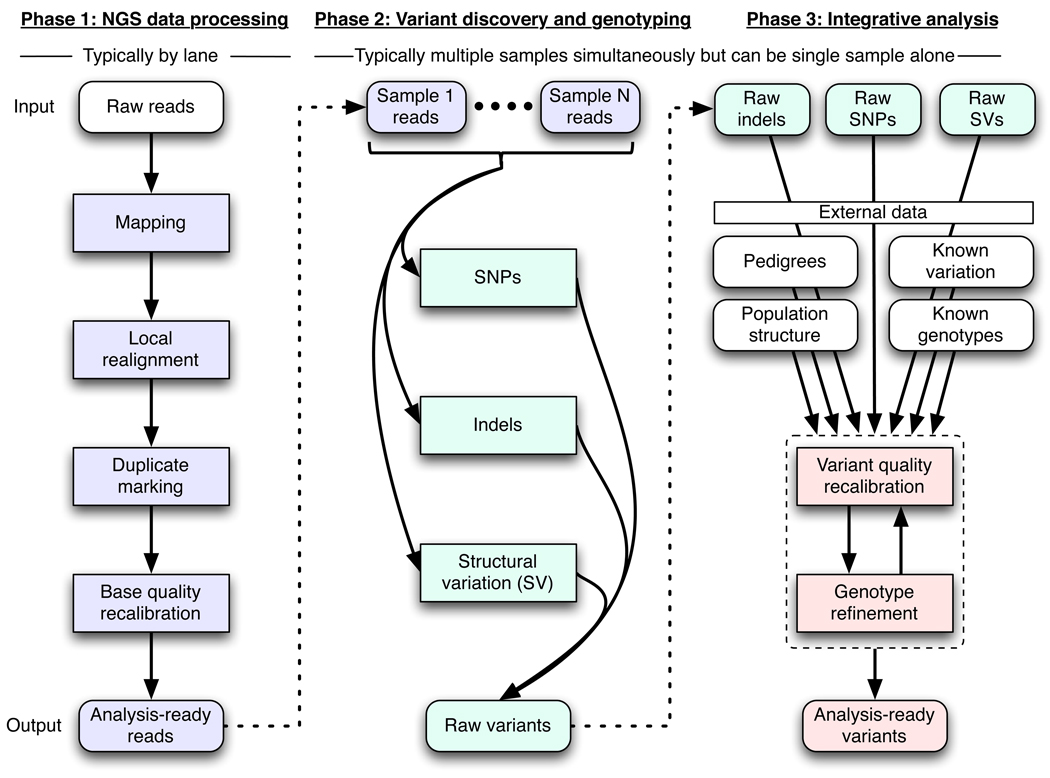
\includegraphics[width=1.0\textwidth]{variationdiscover.jpg}
\caption{Proceso de descubrimiento de variantes en el ADN.\label{fig:procesodescubrimiento}}
\end{figure} 

\section{Descripci�n de un recalibrador}

\section{B�squeda de informaci�n}

\section{Elecci�n de tecnolog�as}
c, sse

\section{Dise�o del software}

\section{Herramientas utilizadas}
geani, git, gdb, valgrind

\section{Evaluaci�n y comparaci�n del recalibrador obtenido}